\vspace{-2mm}
\section{\ouralg: A Program-Aware Agentic Inference System}
\label{sec:thunder_agent}

With all findings in \autoref{sec:motivation}, we present \ouralg, a program-aware system for high throughput agentic inference. We model the Agentic Program in \autoref{sec:program_definition}, which serves as our primary abstraction for scheduling. \autoref{sec:utility_model} formalizes a cost model to guide our system design. Built upon these foundations, we detail our KV cache scheduling policy in \autoref{sec:scheduling_policy} and tool resource management strategy in \autoref{sec:tool_resource}.

\begin{table}[ht]
\caption{\textbf{Summary of Notations for agentic programs.} Each program instance is characterized by its identity, execution phase, tool environments, resource footprint, and scheduling state in \ouralg.}
\vspace{-1.5em}
\label{tab:notations}
\begin{center}
\small
\renewcommand{\arraystretch}{1.1}
\begin{tabularx}{\columnwidth}{lX}
\toprule
\textbf{Notation} & \textbf{Description} \\
\midrule
$P$ & Agentic program instance \\
$\mathit{ID}$ & Unique global identifier for the program \\
$c$ & Number of tokens in the context \\
$\mathcal{T}$ & Set of tool environments required by the program \\
$\mathcal{L}$ & Backend (GPU node) placement for spatial locality \\
$\tau$ & Execution phase: Reasoning (\textbf{R}), \text{Acting (\textbf{A})} \\
$s$ & Scheduling status: $\{\text{Active, Paused, Terminated}\}$ \\
\bottomrule
\end{tabularx}
\end{center}
\vspace{-8mm}
\end{table}

\begin{figure*}[!t]
    \centering
    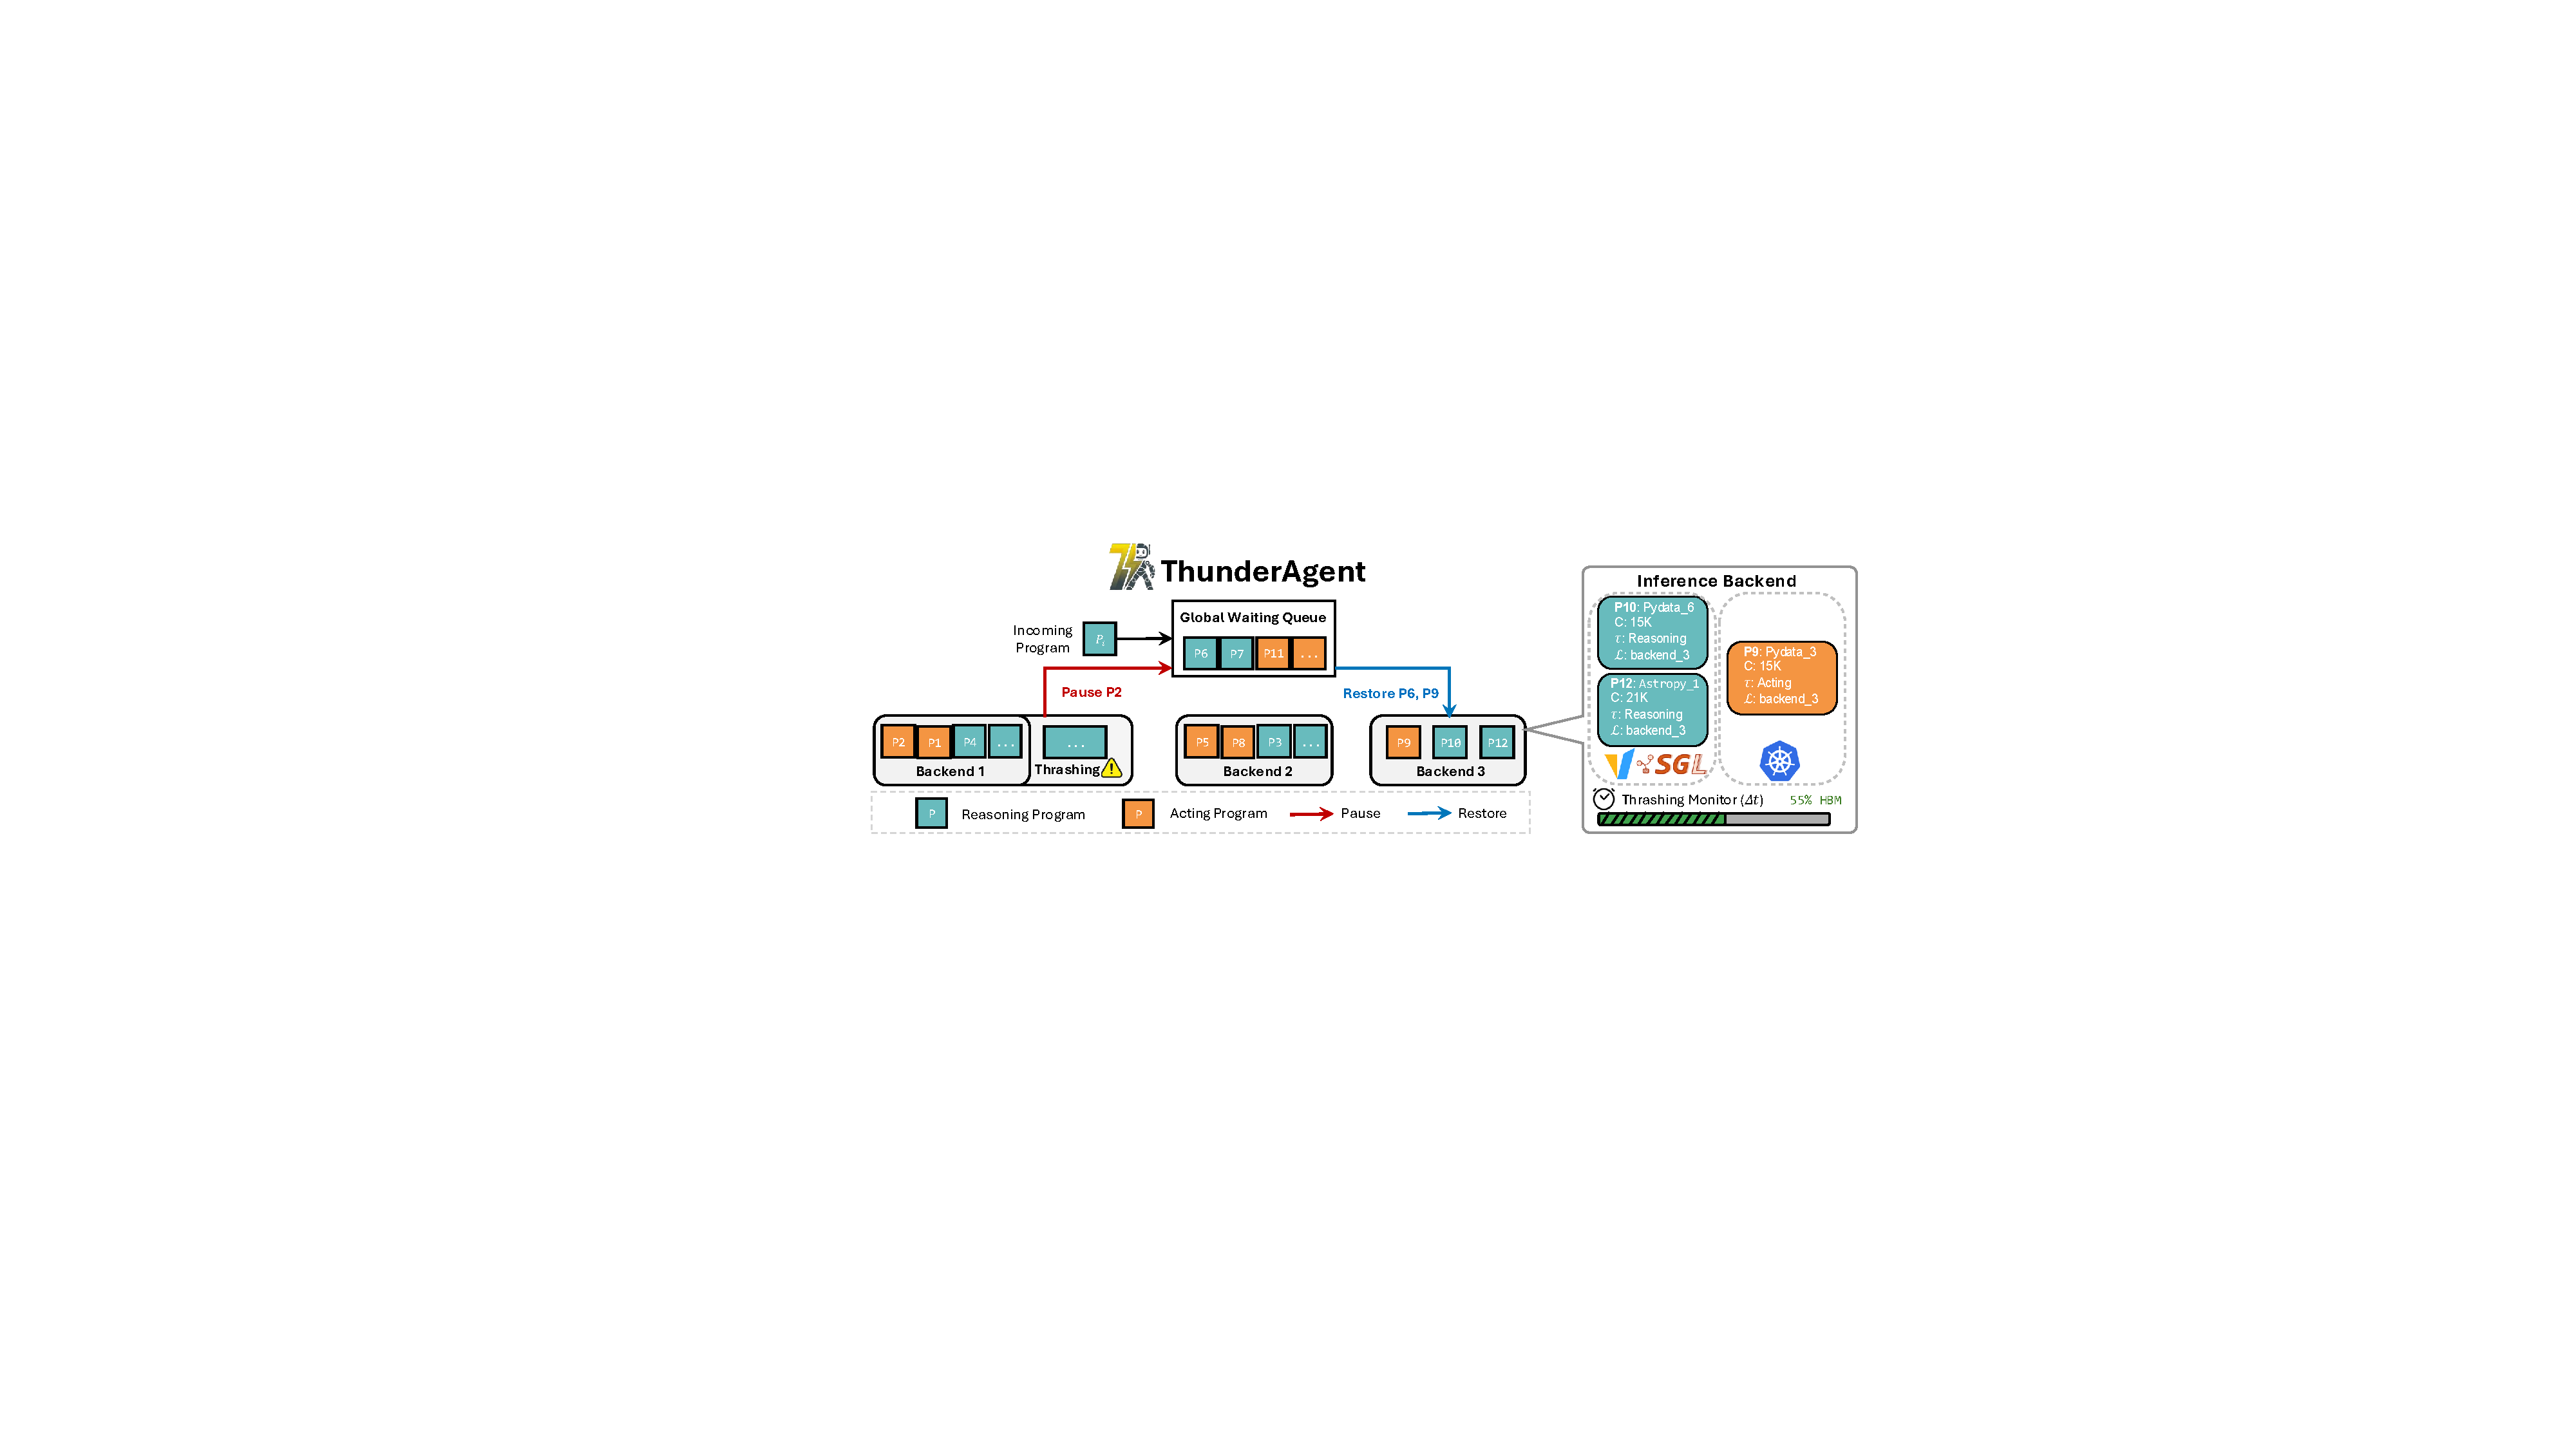
\includegraphics[width=1.0\columnwidth]{Figures/TR5.pdf}
    \caption{\textbf{An Overview of \ouralg.} \textmd{We show the transition between scheduling states and memory management. \ouralg queries the state of each data parallel backend periodically every $\Delta t$ time. Here, Backend \#1 triggers thrashing, while Backend \#3 is underutilized. The global waiting queue shared by all Backends then pauses and collects acting Program \#2 back to the queue while releasing reasoning Program \#6 and \#9, to stop the KV-cache thrashing in Backend \#1 and reduce memory imbalance of Backend \#3.}
    % \junxiong{Should we say Reasoning Phase and Acting Phase instead of Reasoning Program and Acting Program. Because programs switch between reasoning and acting. Readers may get confused and think we don’t have different types of programs.} \junxiong{Need a few sentence to describe this. This figure shows how ThunderAgent manages agent programs across multiple inference backends to avoid KV-cache thrashing. Programs run in per-backend working pools and are labeled as Reasoning or Acting depends on their current execution status. When a backend becomes memory-pressured, ThunderAgent pauses a selected program (red arrow) and moves it into a global waiting queue, freeing HBM and stopping thrashing. When capacity becomes available elsewhere, backends resume programs from the global queue (blue arrow). We prioritize pausing the program in acting (P2) rather than pausing a program in reasoning (P4). }
    }
    \label{fig:arch}
    \vspace{-4mm}
\end{figure*}

% \begin{figure*}[t!]  % 使用 figure* 让图片跨越两栏
%     \centering
%     \begin{subfigure}{0.75\textwidth}
%         \centering
%         \includegraphics[width=0.99\textwidth]{Figures/TR3.pdf}  % 替换为你的图片路径
%         \caption{LMcache offload}
%         \label{fig:kv offload}
%     \end{subfigure}
%     \begin{subfigure}{0.20\textwidth}
%         \centering
%         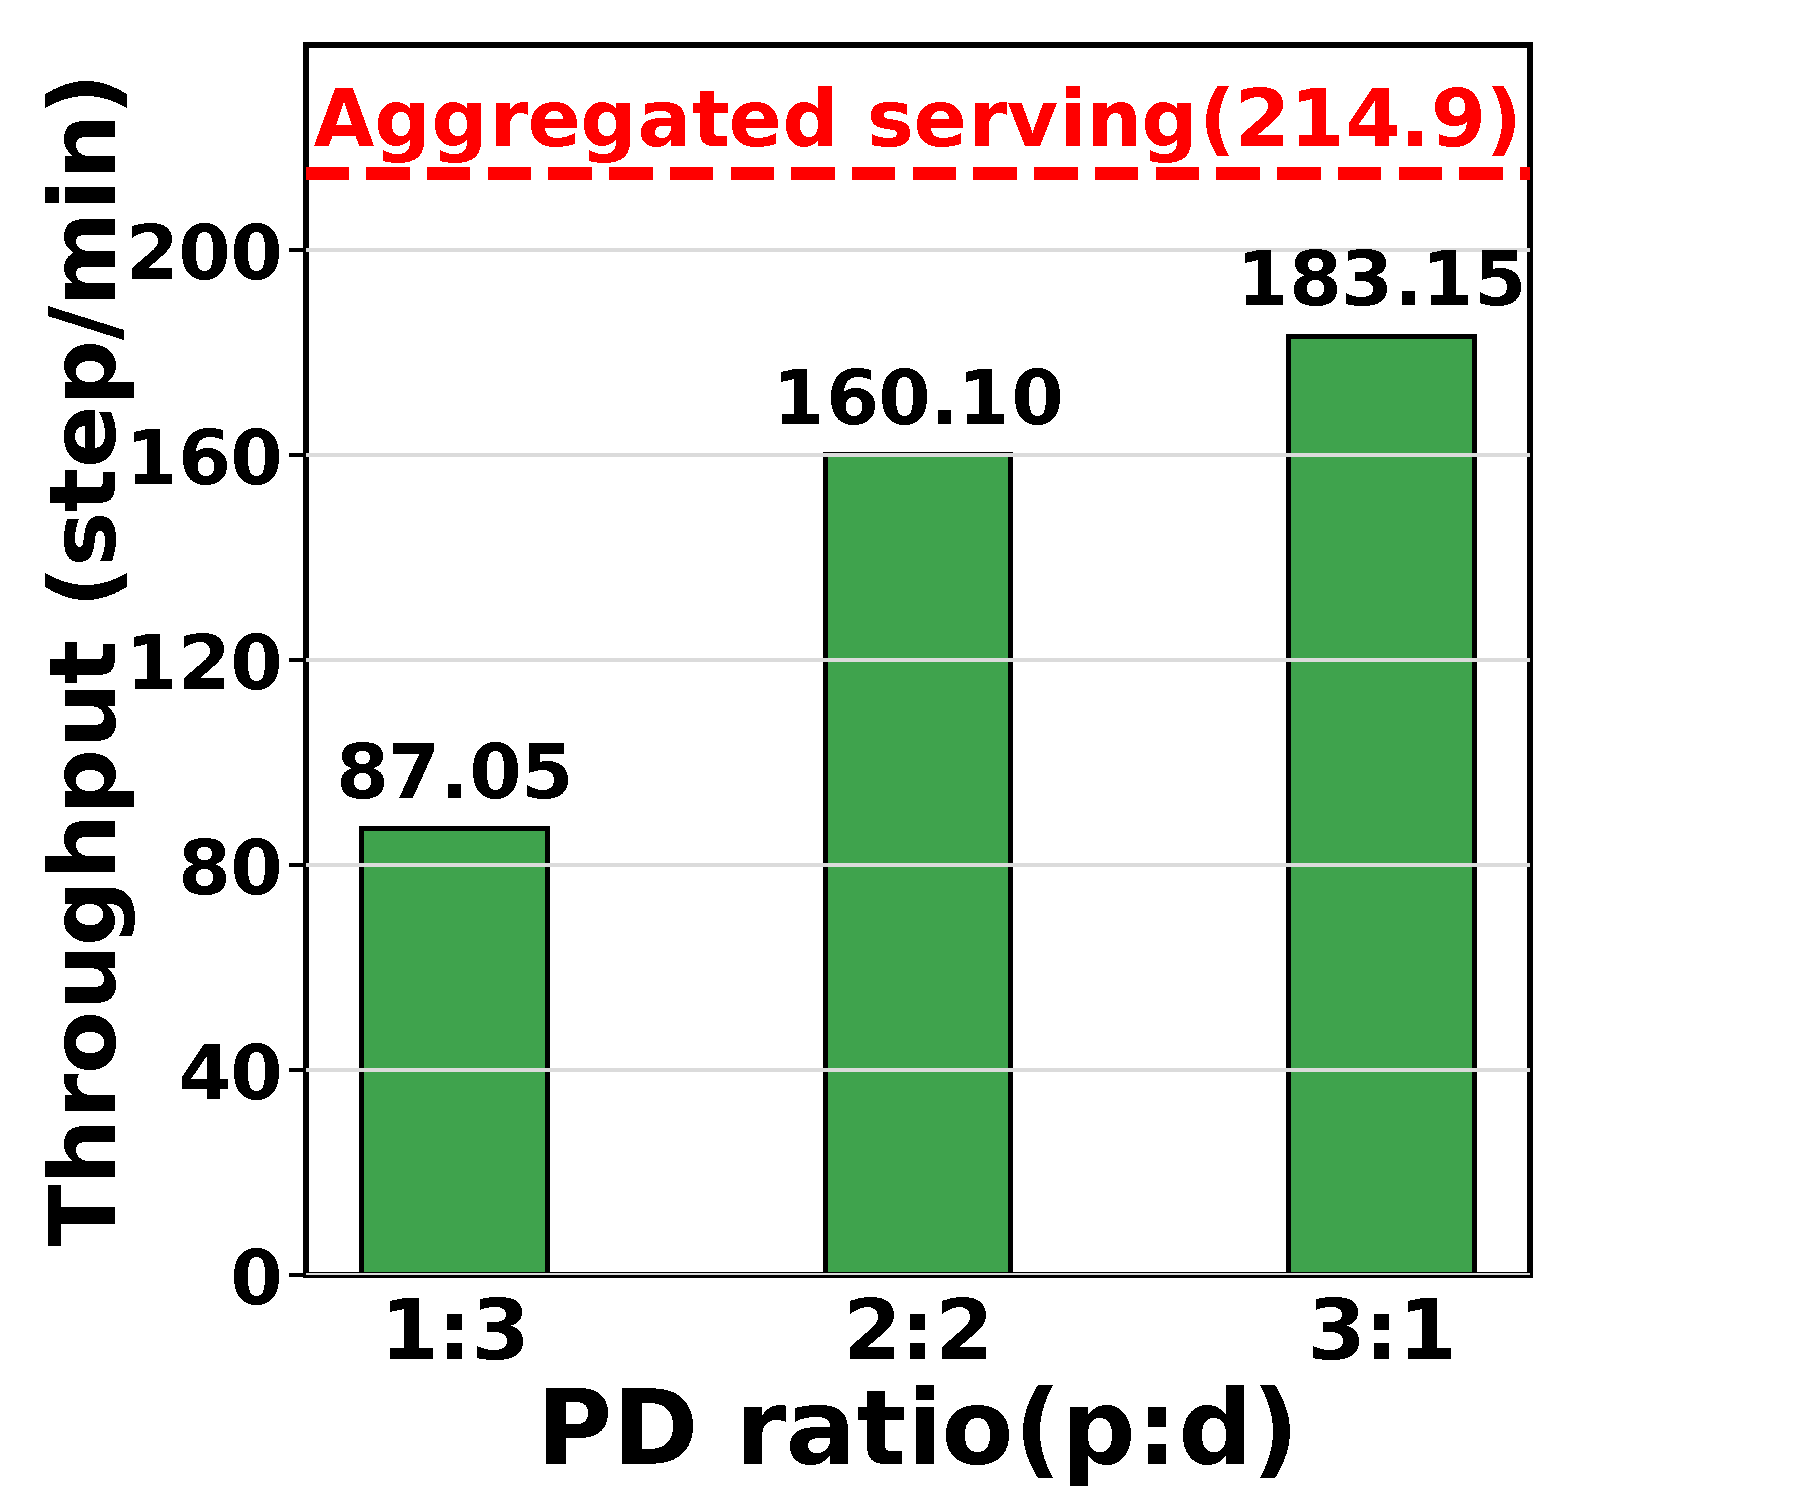
\includegraphics[width=0.99\textwidth]{Figures/throughput_vs_pd_ratio.pdf}  % 替换为你的图片路径
%         \caption{PD Disaggregation}
%         \label{fig:pd disaggregation}
%     \end{subfigure}
%     \vspace*{-0.2mm}
%     \caption{Ablation study of KV cache offload and prefill-decode disaggregation.}
%     \vspace{-4mm}
%     \label{fig:3}
% \end{figure*}
\subsection{Program Abstraction}
\label{sec:program_definition}
The \textbf{Agentic Program} serves as a fundamental abstraction that encapsulates both the logical execution flow and the system-level dependencies of agentic workflows. Formally, we define an agentic program $P$ as a tuple:
\begin{align}
P = \langle \mathit{ID}, c, \mathcal{T}, \mathcal{L}, \tau, s \rangle,
\end{align}
% \vspace{-1mm}
where $\mathit{ID}$ represents the unique global identifier. $c$ denotes the number of tokens in the context, corresponding to the KV cache memory footprint during active execution. $\mathcal{T}$ tracks the set of tool environments used by the program, enabling garbage collection when no program requires them further. $\mathcal{L}$, $\tau$, and $s$ denote the node placement, execution phase, and scheduling status, respectively, facilitating program-level KV cache thrashing \mbox{reduction and cross-node transferring. A metadata example is demonstrated on the right side of \autoref{fig:arch}.}

\ouralg directly wraps existing LLM engines and tool orchestrators by interfacing with OpenAI-style endpoints. Program IDs allow the system to distinguish requests from different agentic workflows. We elaborate on the simplicity of integrating \ouralg with existing inference services in Appendix \ref{app:easy_intergrate}.

\subsection{Cost Model}
\label{sec:utility_model}

During multi-turn agentic inference, only the resources used for active prefilling and decoding contribute to the system's effective throughput, while re-computation, used capacity, and idle caching constitute resource waste. We encompass this in a cost model for GPU resource consumption, which isolates effective costs from non-productive usage. We adopt the Space-Time Product (STP)~\citep{5388441} as our primary metric, defined as the integral of the memory footprint over processing time. The STP cost during a process phase is formalized as:
% \vspace{}
\begin{equation}
    \text{Cost}_{\text{x}} = \int_{0}^{t_{x}} M_x(t) \, dt,
\end{equation}
\noindent where $t_x$ is the duration of process $x$ (e.g., prefill). Since memory usage $M_x(t)$ can be directly quantified by the KV cache token count used in LLMs, we define our cost model as the integral of token count over time.

The total cost of agentic inference comprises five distinct components: decoding, prefilling, recomputation, unused capacity, and idle caching. We explicitly distinguish incremental prefilling for tool execution results from recomputation over historical interactions, with the latter leading to significantly higher cost due to re-computing evicted KV cache over the full context. Formally, this yields the following cost decomposition:
\begin{equation}
    \text{Cost}_{\text{total}} \approx \text{Cost}_{\text{decode}} + \text{Cost}_{\text{prefill}} + \text{Cost}_{\text{recompute}} +
    \text{Cost}_{\text{unused}} + \text{Cost}_{\text{caching}}
    \label{eq:cost_decomp}
\end{equation}
\noindent In this decomposition, $\text{Cost}_{\text{decode}}$ and  $\text{Cost}_{\text{prefill}}$ represents the effective work that contributes to inference throughput. The remaining terms are wasted system overheads: $\text{Cost}_{\text{recompute}}$ stems from KV cache thrashing (\autoref{sec:kv cache management}); $\text{Cost}_{\text{unused}}$ reflects memory imbalance across data parallel (DP) inference backend replicas (\autoref{sec:cross node imbalance}); and $\text{Cost}_{\text{caching}}$ accumulates while holding memory during external tool execution (\autoref{sec:Tool mismanagement}).

\subsection{Scheduling Policy}
\label{sec:scheduling_policy}
Based on the cost model above, the optimization target of our scheduling policy is to minimize the non-productive overhead components: $\text{Cost}_{\text{recompute}}$, $\text{Cost}_{\text{unused}}$, and $\text{Cost}_{\text{caching}}$, thereby maximizing throughput.

\subsubsection{Reducing Recomputation and Caching Costs via Program-Aware Waiting Queue}
\label{sec:4.3.1}
As identified in \autoref{sec:kv cache management} and \autoref{fig:workload_profile}, KV cache thrashing serves as the primary bottleneck for throughput degradation. To address this limitation, the system must minimize $\text{Cost}_{\text{recompute}}$ by explicitly controlling the number of active programs. \ouralg achieves this by introducing a program-aware waiting queue. Our system utilizes this queue to schedule program execution, determining which program should be executed in GPU versus which should be swapped out based on their token length $c$ and execution phase $\tau$. Here, we formalize the scheduler behavior using two primitive operations: \textbf{Restore} and \textbf{Pause}, as follows.

\begin{itemize}[itemsep=0.0pt,topsep=0pt,leftmargin=*]
    \item \textbf{Restore.} This operation admits a program into active execution. Given a program $P = \langle \mathit{ID}, c, \mathcal{T}, \mathcal{L}, \tau, s \rangle$ with $s = \text{Paused}$ and $\mathcal{L} = \varnothing$,
  Restore$(P)$ assigns $P$ to a backend $\mathcal{L}'$ with available capacity and updates
  \begin{align}
  P \leftarrow \langle \mathit{ID}, c, \mathcal{T}, \mathcal{L}', \tau, \text{Active} \rangle,
  \end{align}
    \item \textbf{Pause.} This operation removes a program from active execution.
Given a program $P = \langle \mathit{ID}, c, \mathcal{T}, \mathcal{L}, \tau, s \rangle$
with $s = \text{Active}$,
Pause$(P)$ unbinds $P$ from its backend, releases its KV cache for preemption, and updates
\begin{align}
P \leftarrow \langle \mathit{ID}, c, \mathcal{T}, \varnothing, \tau, \text{Paused} \rangle .
\end{align}
\end{itemize}

\noindent Building on these two operations, we next introduce our scheduling policy to minimize KV cache thrashing.

\paragraph{Periodic thrashing detection.}  The program abstraction in \autoref{sec:program_definition} provides us with the KV cache size of acting programs. Notably, this is unavailable in request-level systems (as in \autoref{sec:motivation}). We define the thrashing condition for a DP backend $\mathcal{L}$ as the state where program memory demand exceeds total capacity:
\begin{equation}
    \text{C}_{\text{total}} < \sum_{p \in \mathcal{L}} c_p
\end{equation}
\noindent where $\text{C}_{\text{total}}$ denotes the fixed token capacity of the KV cache pool for backend $\mathcal{L}$. During decoding, the context length $c_p$ of agentic workflows grows rapidly, which can trigger memory thrashing \emph{mid-execution} even without of new arrivals. Unlike baseline schedulers (e.g., Continuum) that only perform checks on whether to admit a workflow upon its arrival, we implement a \textbf{periodic monitor} that evaluates the memory usage at fixed intervals $\Delta t$, \mbox{allowing preemptive detection and mitigation of memory pressure caused by context growth.}

When KV cache thrashing is imminent, \ouralg invokes \textbf{Pause} operation to suspend active programs and free memory size $\Delta C = \sum_{p \in \mathcal{L}} c_p - \lambda_{\max} \cdot \text{C}_{\text{total}}$ until the total memory usage falls below the limit $\lambda_{\max} \cdot \text{C}_{\text{total}}$. Conversely, when the backend has available space, meaning
$\sum_{p \in \mathcal{L}} c_p < \lambda_{\min} \cdot C_{\text{total}}$, \ouralg restores paused programs from the waiting queue via \textbf{Restore}, ensuring that the restored program keeps the total memory below $\lambda_{\max} \cdot \text{C}_{\text{total}}$. Here, $\lambda_{\max}$ and $\lambda_{\min}$ denote the high- and low-watermarks
of memory usage, respectively, together forming a hysteresis window that
stabilizes our scheduling. In practice, we set both value to be 1, as the shared prompt across programs implicitly reserves sufficient memory buffer.

With this program-level periodic capacity check, \ouralg can guarantee that there will be no KV cache thrashing by reserving memory for active programs during the acting phase. However, the tradeoff is that when programs engage in long-running tool execution, the GPU memory occupied by acting programs is idle. To balance the cost of caching against recomputation, we incorporate a time-decay mechanism into the thrashing check that progressively discounts the effective weight of acting programs' tokens. This allows the scheduler to evict long-idling caching when memory pressure rises, rather than holding them indefinitely:
\begin{equation}
\label{eq:time_decay}
    \text{C}_{\text{total}} < \sum_{p \in \mathcal{L},\tau = \textbf{R}} c_p +\sum_{q \in \mathcal{L},\tau = \textbf{A}} c_q \times f(t_q)
\end{equation}
Specifically, $t_q$ is the tool execution time of program $q$ in the current step. $f(t)$ is a time-decay function designed to balance $\text{Cost}_{\text{caching}}$ and $\text{Cost}_{\text{recompute}}$. By dynamically lowering the effective memory priority of acting programs over time, $f(t)$ encourages the scheduler to evict caches that remain idle.
In \autoref{app:ft_discussion}, we prove that when tool execution latencies satisfy the memoryless property (i.e., the remaining execution time is independent of the elapsed duration), the optimal decay function $f(t)$ takes the form of exponential decay.

\paragraph{Minimizing $\text{Cost}_{\text{recompute}}$ via Shortest-First Eviction.}
With the eviction and restoration conditions above, the remaining question in handling thrashing is to determine which subset of active programs to pause such that the recomputation cost is minimized. In this paragraph, we demonstrate that evicting programs with the smallest KV cache size yields the optimal solution, with a detailed proof provided in \autoref{app:prefill_stpcost}.

\begin{lemma}[Quadratic Recomputation Cost]
\label{lem:recompute_quadratic}
Given  a program $P_i$ with context length $c_i$, the recomputation cost incurred by reprefilling its KV cache scales quadratically with $c_i$, i.e.,
\begin{equation}
    \text{Cost}_{\text{recompute}} = \int_{0}^{t_{\mathrm{recompute}}} c_i(t) \, dt \propto c_i^2.
\end{equation}
\end{lemma}

\begin{definition}[Eviction Optimization Problem]
\label{def:eviction_problem}
Based on Lemma~\ref{lem:recompute_quadratic}, given a required memory release $\Delta C$, the scheduler aims to
select a subset $S$ of programs to evict such that the released
capacity satisfies the constraint while minimizing the total
recomputation cost. This optimization problem is formulated as follows:
\begin{equation}
\min_{S} \sum_{i \in S} c_i^2
\quad \text{s.t.} \quad
\sum_{i \in S} c_i \ge \Delta C.
\end{equation}
\end{definition}

The objective is strictly minimized by selecting smaller $c_i$.  Thus, \ouralg's strategy is to greedily pause and evict programs with the \textbf{shortest context lengths}. We defer the formal proof to Appendix~\ref{app:_minimized_STP_cost}. Based on these analyses, we employ the following scores for restoring and pausing a program in our scheduler:
\begin{equation}
    S_{\mathrm{restore}}(P) = \frac{1}{c_P} + \mathbb{I}(\tau = \textbf{R})
\end{equation}
\begin{equation}
    S_{\mathrm{pause}}(P) = \frac{1}{c_P} + \mathbb{I}(\tau = \textbf{A})
    \end{equation}
\noindent where the indicator function $\mathbb{I}(\cdot)$ enforces strict prioritization of the program's execution state ($\tau$) over context length. Both mechanisms follow the \textbf{shortest-first} policy to minimize recomputation cost. However, the state indicator $\mathbb{I}$ ensures that the scheduler prioritizes pausing Acting programs, thereby minimizing $\text{Cost}_{\text{caching}}$ by reclaiming cached memory, while prioritizing restore Reasoning programs to maximize $\text{Cost}_{\text{decode}} + \text{Cost}_{\text{prefill}}$.

\subsubsection{Reducing Memory Imbalance via Global Program-Aware Waiting Queue}
\autoref{sec:kv cache management} and \autoref{fig:dp unbalance} highlight that memory imbalance across nodes introduces significant $\text{Cost}_{\text{unused}}$, leading to unnecessary program pausing despite sufficient memory capacity from other nodes. To this end, \ouralg unify waiting queues of all backend replicas into a \textbf{global program-aware waiting queue}.

The key motivation of this design is that $\text{Cost}_{\text{unused}}$ arises only
when paused programs remain in the waiting queue while some replicas
have idle memory. Moreover, once a program is paused, its KV cache is
assumed to be evicted, making its recomputation cost node-agnostic. This allows us to improve cross-node memory balance without sacrificing KV cache locality. The restore policy aligns with load balancing rather than strict KV-aware routing, enabling paused programs to be dispatched to any
replica with available memory capacity. As a result, the global queue bounds the unused cost such that $\text{C}_{\text{unused}} < c_{\mathrm{min}} \cdot \Delta t$\footnote{Since $\Delta t$ is much smaller than a program’s lifetime, we ignore the impact of terminated programs within a single interval.} for every node in the period of $\Delta t$, where $c_{\mathrm{min}}$ represents the minimum token length among paused programs. An overview of the scheduling policy and the global waiting queue in \ouralg is presented in \autoref{fig:arch}.

\subsection{Tool Resource Management}
\label{sec:tool_resource}
Next, \ouralg mitigates the resource leakage and environment setup overheads detailed in \autoref{sec:Tool mismanagement}.
% , using the program-aware abstraction.
\paragraph{Hook-based garbage collection.} We implement lifecycle hooks that strictly couple the persistence of tool resources with the agentic program's scheduling status $s$. When a program is \textit{Terminated}, the collector triggers an immediate teardown sequence, systematically reclaiming sandboxes, network sockets, and compute slots. The active disk usage in \autoref{fig:disk mem} showcases that our resource management policy effectively prevents the accumulation of excessive resources, maintaining a near-constant disk memory consumption over time.


\paragraph{Asynchronous environment preparation.} The latency involved in initializing a tool execution environment
 (e.g., starting a Docker container and installing dependencies) can be a bottleneck. To address this, \ouralg monitors the global waiting queue; when a high-priority program (high $S_\text{restore}$) approaches the restore threshold, the system asynchronously restores its execution environment before the GPU memory is allocated. This technique effectively \textbf{hides the initialization overhead}, significantly reducing end-to-end latency for tool-call heavy workloads like coding agents and science agents, as demonstrated in \autoref{fig:env prepare}.